\chapter{Method}\label{ch:method}

The problem can generally be described as a classification problem, where an algorithm tries to predict the label or class of some input features.
For this thesis the input is the document representation in the form of text embeddings, which are labeled with the nominal stock price change, that the report created, so \textit{positive} or \textit{negative}.

\section{Overview of machine learning algorithms}
All these algorithms have in common, that they take a n-dimensional input vector to predict m classes.
Mathematically this can be seen as a function $f(x)=y$ with $x\in\mathbb{R}^n$ and $y\in\{0, 1\}$, since it is a binary classification problem.
The algorithms are able to find patterns in the data and can autonomously improve their prediction performance.
This learning process requires a training phase.
This section addresses the different machine learning algorithms used in the research which are the Naive Bayes classifier, the \acl{KNN} classifier, the \acl{SVM} and the \acl{LSTM} as well as the method to create document embeddings.
\subsection{Naive Bayes classifiers}
The idea behind the Naives Bayes classifier is, that certain input features correlate with a certain class, which means that these input features result with a high probability from this certain class.
The Naive Bayes classifier makes use of the assumption, that each feature of the input vector is independent to one another.
Using the Bayes theorem (equation \ref{equation:bayes}), the Naive Bayes classifier can compute the probability of a class given the features of the input.
\begin{equation}
    P(Y|X) = \frac{P(X|Y)P(Y)}{P(X)}
    \label{equation:bayes}
\end{equation}
% During training the algorithm has to determine the probabilities on the right side of the equation $P(X|Y), P(Y)$ and $P(X)$.
The probability $P(Y)$ is given by the proportion of a class in the whole training dataset.
For a balanced dataset with two classes this gives the probabilities $P(y_1, y_2)=\langle0.5,0.5\rangle$.
% $P(X|Y)$ is given by $P(X|Y)=\frac{P(X \implies Y)}{P(Y)}$.
Determining $P(X|Y)$ is not as trivial:
Since $X$ can be a vector $(x_1, x_2, ..., x_n)$ of variables, it would be necessary to determine $P(x_1 \land x_2 \land ... \land x_n|Y)$ for all combinations of $x_i$, which would require $O(2^n)$ space to save the values and make it impossible to use the algorithm with high dimensional input \cite[p. 493]{Russel2016}.
The assumption that $x_1, ..., x_n$ are independent, however, simplifies this problem.
$P(x_1 \land x_2 \land ... \land x_n|Y)$ can now be decomposed into $P(x_1|Y)\cdot P(x_2|Y)\cdot...\cdot P(x_n|Y)$ which only requires $O(n)$ to save the conditional probabilities and allows for practical usage of the algorithm \cite[p. 499]{Russel2016}.
So during training the algorithm has to determine $P(Y)$ and $P(x_1|Y), P(x_2|Y) ... P(x_n|Y)$.
The probability $P(X)$ is a normalization factor which is chosen so that $P(y_1|X)+P(y_2|X)=1$ \cite[p. 493]{Russel2016}.
During prediction phase $P(Y|X)$ is computed for all classes and the class with the highest probability given $X$ will be the classification result: $y_pred = arg max_i P(y_i|X)$
Even though the assumption, that the features are independent to one another is generally not true, the Naive Bayes classifier often performs equally or even better than more complex methods \cite[p. 211]{Hastie2009}.
For this research, the Naive Bayes implementation from scikit-learn was used in combination with the learning curve generator of the library.

\subsection{\acl{KNN} classifiers}
As the name of this method implies, a nearest neighbor classifier makes its predictions based on the surrounding data points.
Because every input to this classifier can be seen as a point in a n-dimensional space, the \ac{KNN} can compute the distances to other points.
The distance can be measured as Euclidean distance, however other distance metrics are also possible.
Scikit-learn's \texttt{KNeighborsClassifier} for example, measures the distance with the Minkowski distance, which is a generalisation of the Euclidean distance.\footnote{\url{https://scikit-learn.org/stable/modules/generated/sklearn.neighbors.KNeighborsClassifier.html}}
\begin{equation}
    % d_{ab} = \left(\sum_{i=1}^n \abs{a_i - b_i} ^p \right)^{\frac{1}{p}}
    d(x_1, x_2) = \left(\sum_{i=1}^n \abs{x_{1,i} - x_{2,i}} ^p \right)^{\frac{1}{p}}
\end{equation}
The Minkowski distance collapses to the Euclidean distance for $p=2$ and to the Manhatten distance for $p=1$ \cite[p. 738]{Russel2016}.
The predicted class is then the most common class of all $k$ neighbors.
Because the \ac{KNN} classifier makes use of a geometric property of the input data, it is important to scale each feature to have a mean of zero and a variance of one \cite[p. 465]{Hastie2009}.
The optimum $k$ can be found with cross validation, which is described in section \ref{subsec:cross_validation}.

In this thesis the \ac{KNN} implementation from scikit-learn was used as well as the \texttt{StandardScaler} to scale the features.
% In scikit-learn this is done with the \texttt{StandardScaler}.
$k$ was determined by creating a validation curve, which shows how the accuracy changes for different values of $k$.
It is implemented with the code in listing \ref{py:knn_validation_curve}.
The results of this finding are presented in chapter \ref{ch:experiments}.
\lstinputlisting[language=Python,caption={Creates data for a validation curve},captionpos=b, label={py:knn_validation_curve}]{listings/knn_validation.py}
The \texttt{knn\_\_n\_neighbors} argument tells the \texttt{validation\_curve} function, which parameter it should test for the provided estimator.
In this case the estimator is a pipeline, which wraps the \texttt{StandardScaler} and the \texttt{validation\_curve} and executes them sequentially for every fold.
The number of the folds for the cross validation is set with the \texttt{cv} argument.

\subsection{\acl{SVM}s}
A \ac{SVM} tries to fit a decision boundary between the points of two classes, so that the surrounding margin is maximized.
This decision boundary can mathematically be seen as a hyperplane in the n dimensional space of the data points.
For a two dimensional space that results in a line:
\begin{figure}[h]
    \centering
    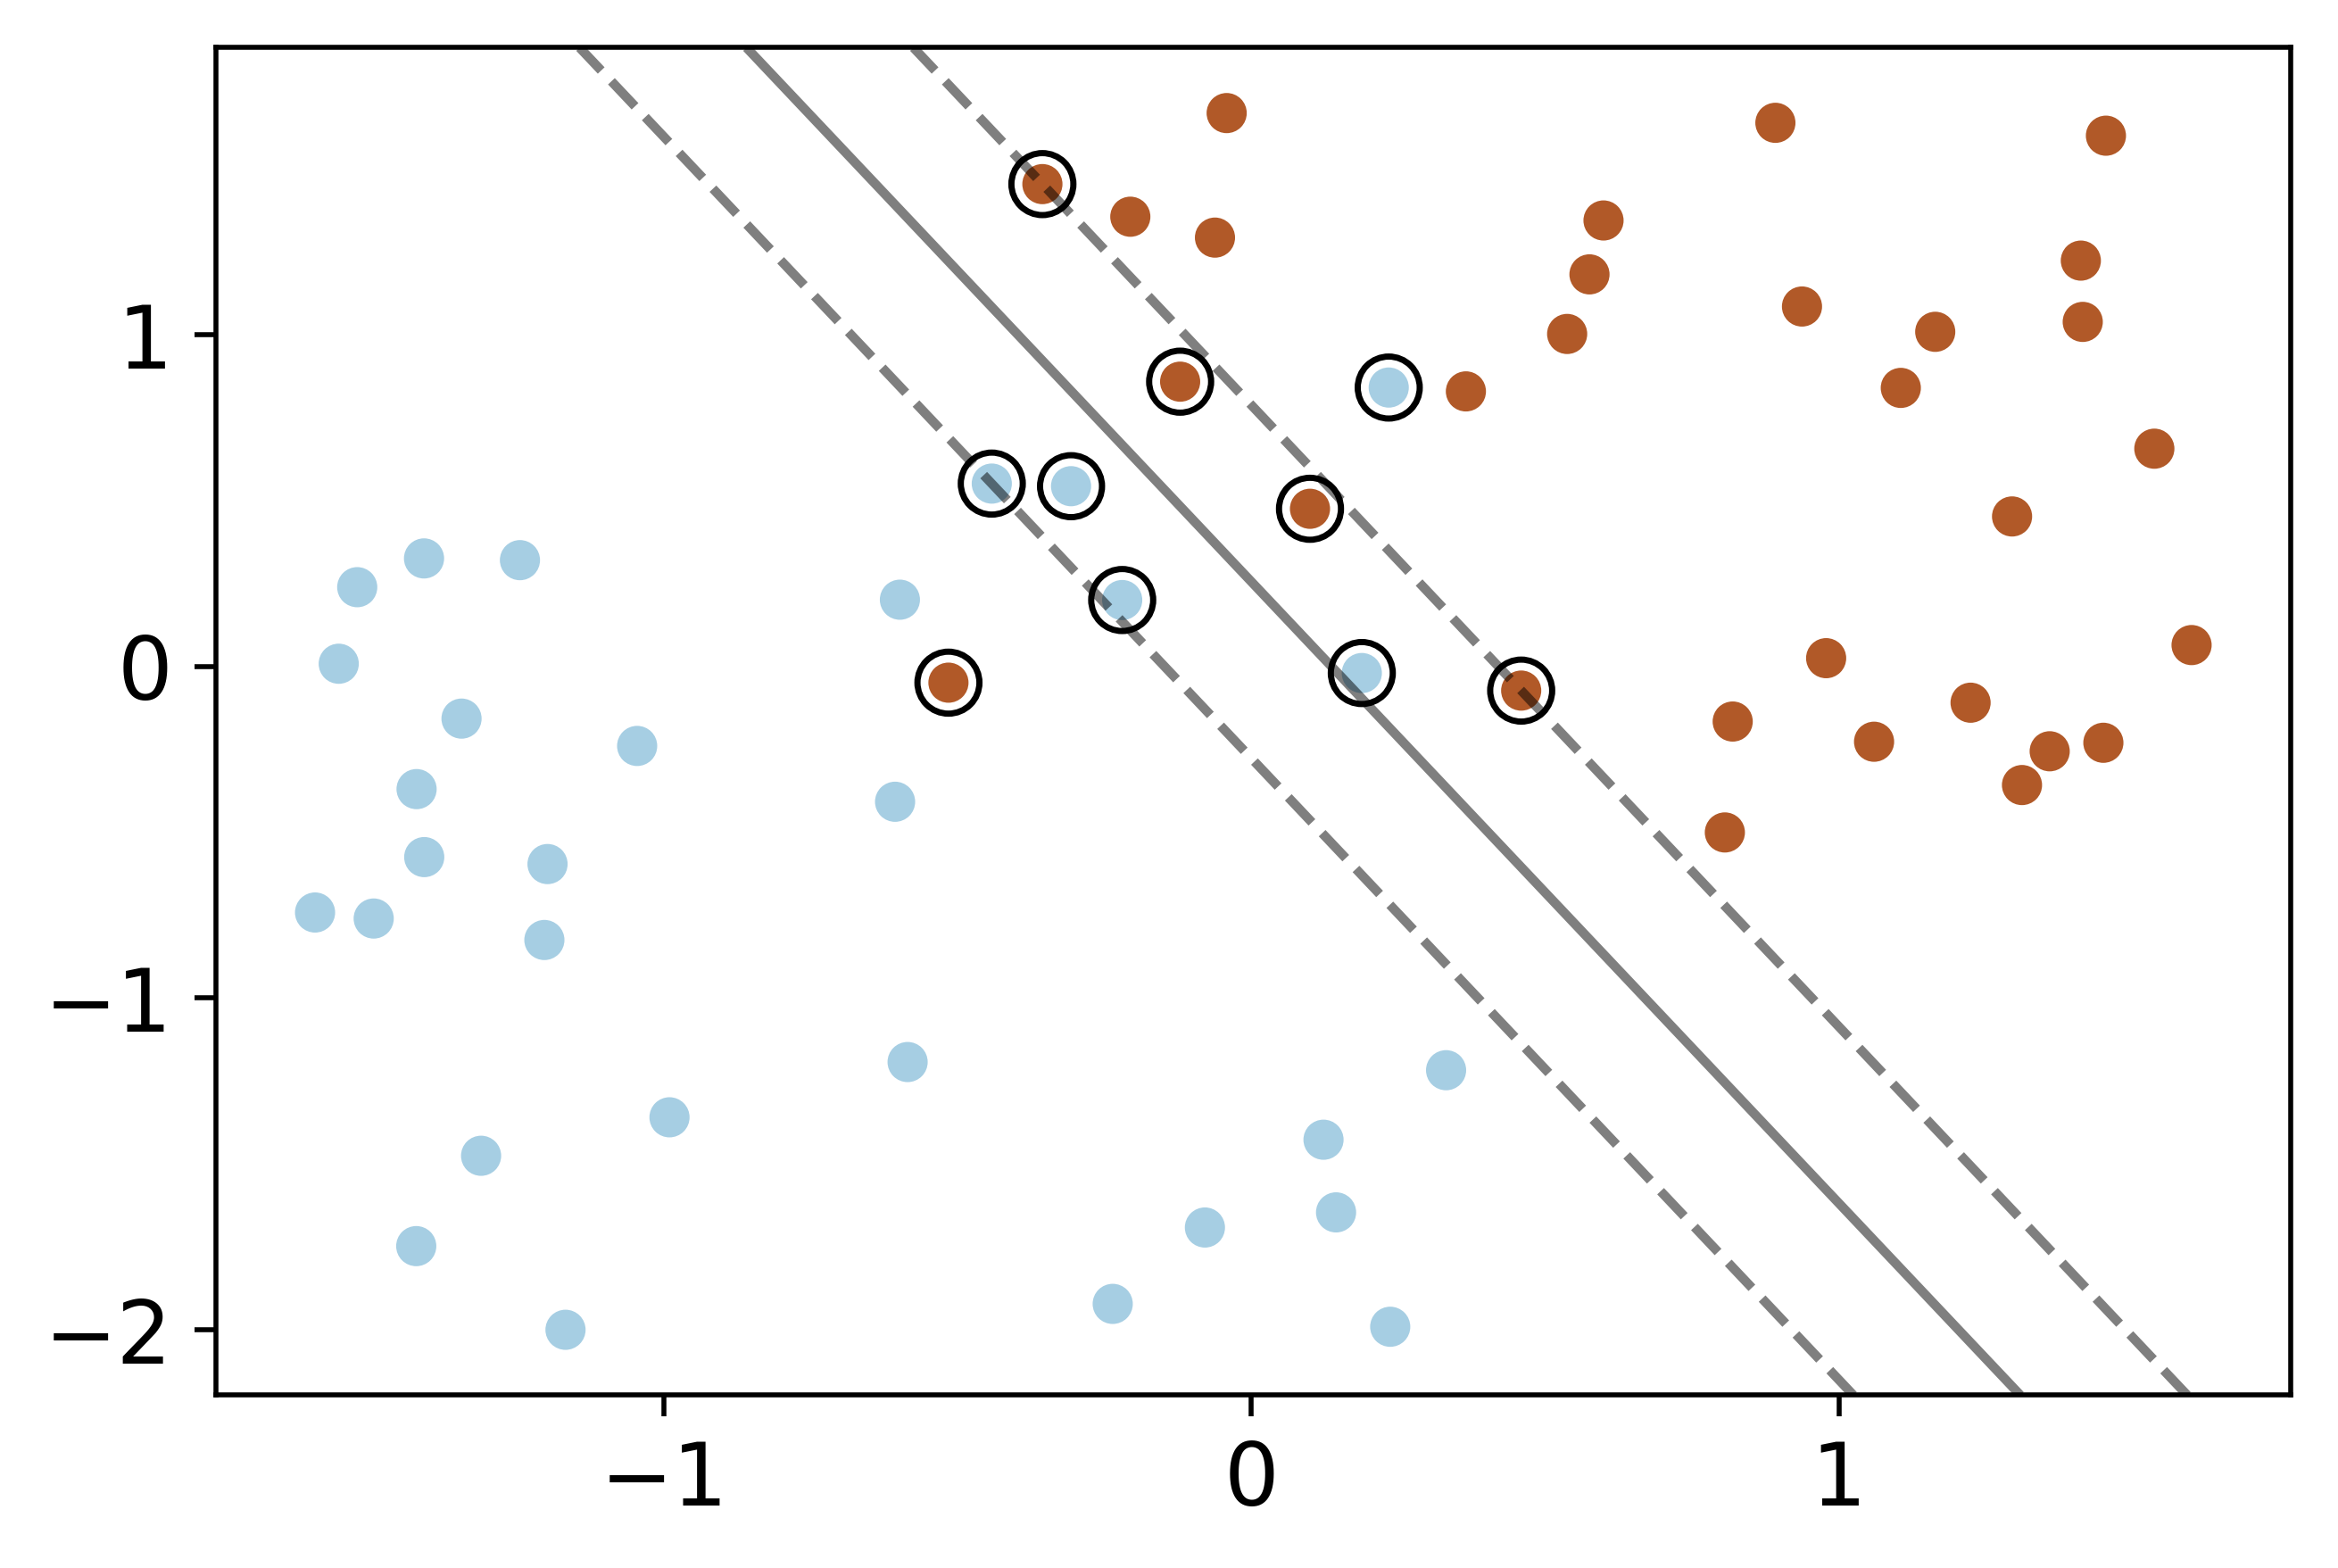
\includegraphics[width=0.5\textwidth]{figures/svm_decision_boundary.png}
    \caption{A decision boundary with its support vectors.\protect\footnotemark}
    \label{figure:svm_decision_boundary}
\end{figure}
\footnotetext{A modified version of the example on scikit-learn: \url{https://scikit-learn.org/stable/auto_examples/svm/plot_separating_hyperplane.html}}
The line in figure \ref{figure:svm_decision_boundary} represents the decision boundary and the dashed lines mark the borders of the margin with maximum width, respecting some constraints which will be discussed in this section.
The circled points mark the \textit{support vectors} which are used to determine the hyperplane.
% This allows the \ac{SVM} to generalize well \cite[p. 744]{Russel2016}.
The decision boundary is mathematically a hyperplane defined by:
\begin{equation}
    f(x)=x^T\beta + \beta_0=0
    \label{equation:svm_hyperplane}
\end{equation}
where $\beta$ is a unit vector, $x_i \in \mathbb{R}^n$ are the sample points and $y_i \in \{-1, 1\}$ are the labels to these points.
Therefore the aim is to maximize the margin between the training points and the hyperplane, which can be re-expressed as
% \begin{multline}
%     max_{\beta, \beta_0, \norm{\beta}=1} M \\ subject to y_i(x_i^T \beta + \beta_0) \geq M, i = 1, ..., N
% \end{multline}
% Mathematically this can be expressed in the form:
\begin{multline}
    min_{\beta, \beta_0}\frac{1}{2}\abs{\abs{\beta}}^2 + C\sum_{i=1}^N\xi_i \\
    subject to \xi_i \geq 0, y_i(x_i^T\beta + \beta_0)\geq 1 - \xi_i \forall i
\end{multline}
where $\xi_i$ is a penalty term, that increases with the distance a data point $x_i$ lies on the wrong side of its margin \cite[p. 7]{Fletcher2008}.
Since this penalty terms are weighted by the constant $C$, the width of the margin varies with choosing the value of $C$.
If $C$ is set really low, a broad margin with many support vectors is used.
If it is set high, only points near the decision boundary are used as support vectors \cite[p.421]{Hastie2009}.
This optimization problem can be solved using Lagrange multipliers and gives for $\beta$
\begin{equation}
    \beta = \sum_{i=1}^{N} \alpha_i y_i x_i
\end{equation}
and for $\beta_0$
\begin{equation}
    \beta_0 = \frac{1}{N_S} \sum_{i=1}^{N_S}(y_i - \sum_{j=1}^{N_S} \alpha_j y_J x_i^T x_j)
\end{equation}
$\alpha$ is the Lagrange multiplier which is $0 < \alpha \leq C$ for all \textit{support vectors} and $0$ for all other points \cite[p. 746]{Russel2016}.
Its exact value can be determined with the dual Lagrangian function of equation \ref{equation:svm_hyperplane} \cite[p. 9]{Fletcher2008}.

The \ac{SVM} as defined so far, has the drawback, that it only creates linear decision boundaries.
Often the classes are not linearly seperable, so a mathematical trick is used, that the \ac{SVM} can still perform on such data.
This is done with a kernel function, which maps the data points to a enlarged feature space.
% $\xi_i$ are the \textit{support vectors}.
% The support vectors are the points that are used to build up the decision boundary, so that it has a maximum distance to them.
% If the classes are linearly seperable, these are the closest points of one class to the other class.
% If the data points of both classes overlap, the support vectors are constructed from the points of one class that lie in the decision region of the other class.
% $C$ is the parameter which sets the width of the margin, if it is set really low, a broad margin with many support vectors is used.
% If it is set high, only points near the decision boundary are used as support vectors.
A way to find decision boundaries for data which is not linearly seperable is to enlarge the feature space with a kernel function.
Thus the data becomes linearly seperable in the enlarged feature spaces, which has the effect of nonlinear boundaries in the original space \cite[p.423]{Hastie2009}.
One typical kernel function is the \textit{Radial Basis Kernel} which has the following form:
\begin{equation}
    K(x_i, x_j) = e^{-\left(\frac{\abs{\abs{x_i - x_j}}^2}{2\sigma^2}\right)}
\end{equation}
The kernel function is used in the dual Lagrangian function of equation \ref{equation:svm_hyperplane}, which is then again optimized.
This has the implicit effect, that the datapoints are mapped to a higher dimensional feature space.
Figure \ref{figure:kernel_3d} shows this mapping to a three-dimensional space with the hyperplane, that seperates the classes, figure \ref{figure:kernel_decision_boundary} shows the base feature space with the resulting circular decision boundary.
\begin{figure}[h]
    % \centering
    \subcaptionbox{Datapoints with a circular decision boundary, resulting from the kernel trick.\label{figure:kernel_decision_boundary}}[0.5\linewidth]{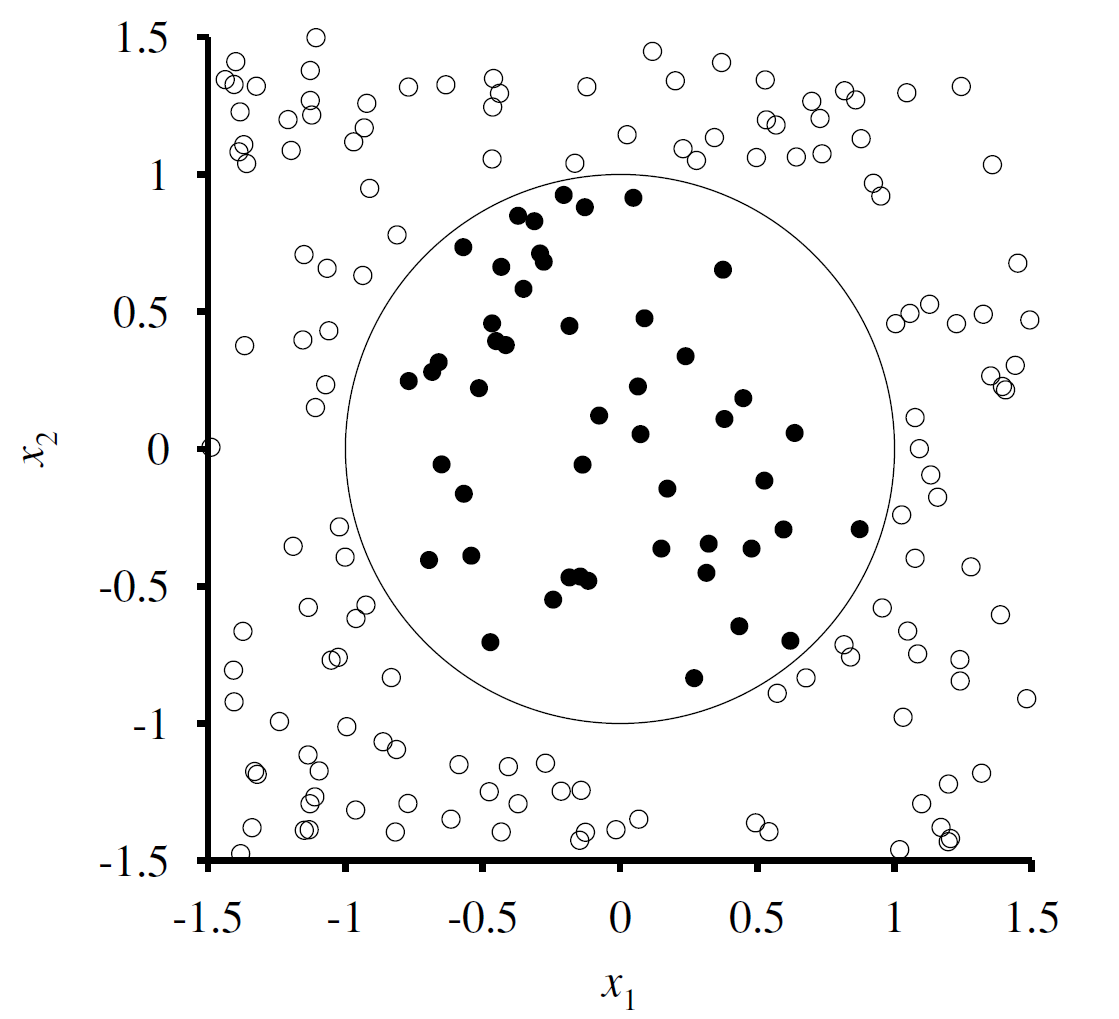
\includegraphics[width=0.5\textwidth]{figures/svm_circular_decision_1.png}}
    \subcaptionbox{When mapped to a higher dimensional space, the datapoints become linearly seperable.\label{figure:kernel_3d}}[0.5\linewidth]{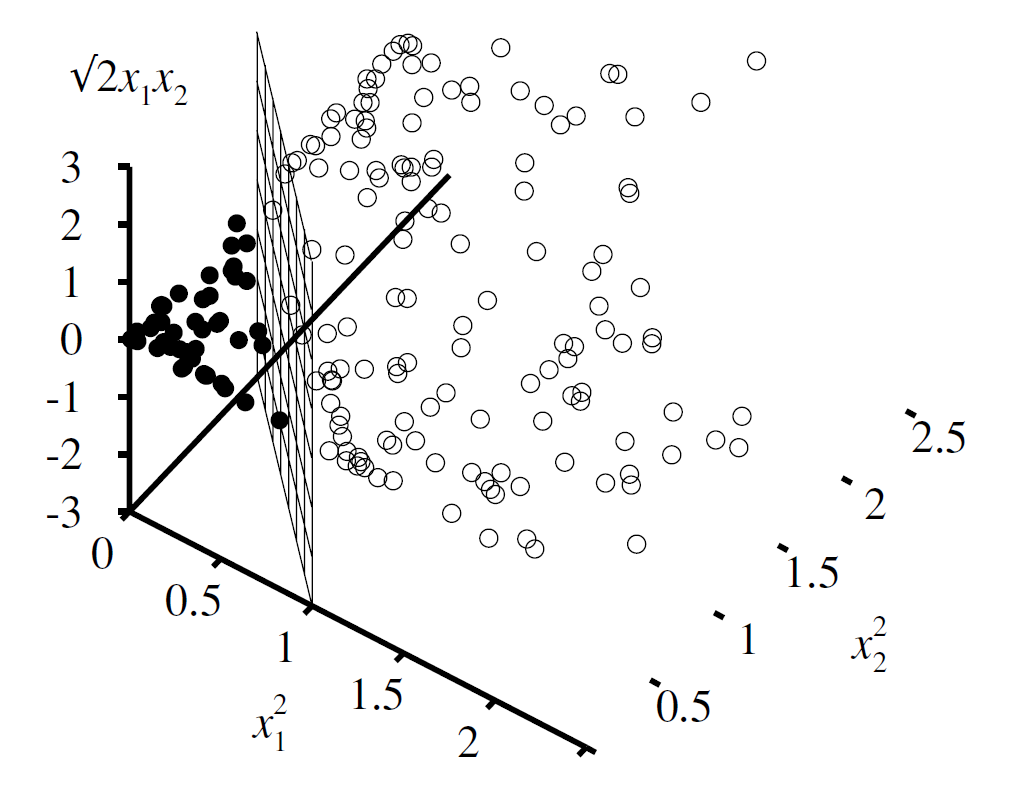
\includegraphics[width=0.5\textwidth]{figures/svm_circular_decision_2.png}}
    % \begin{subfigure}{0.5\textwidth}
    %     \centering
    %     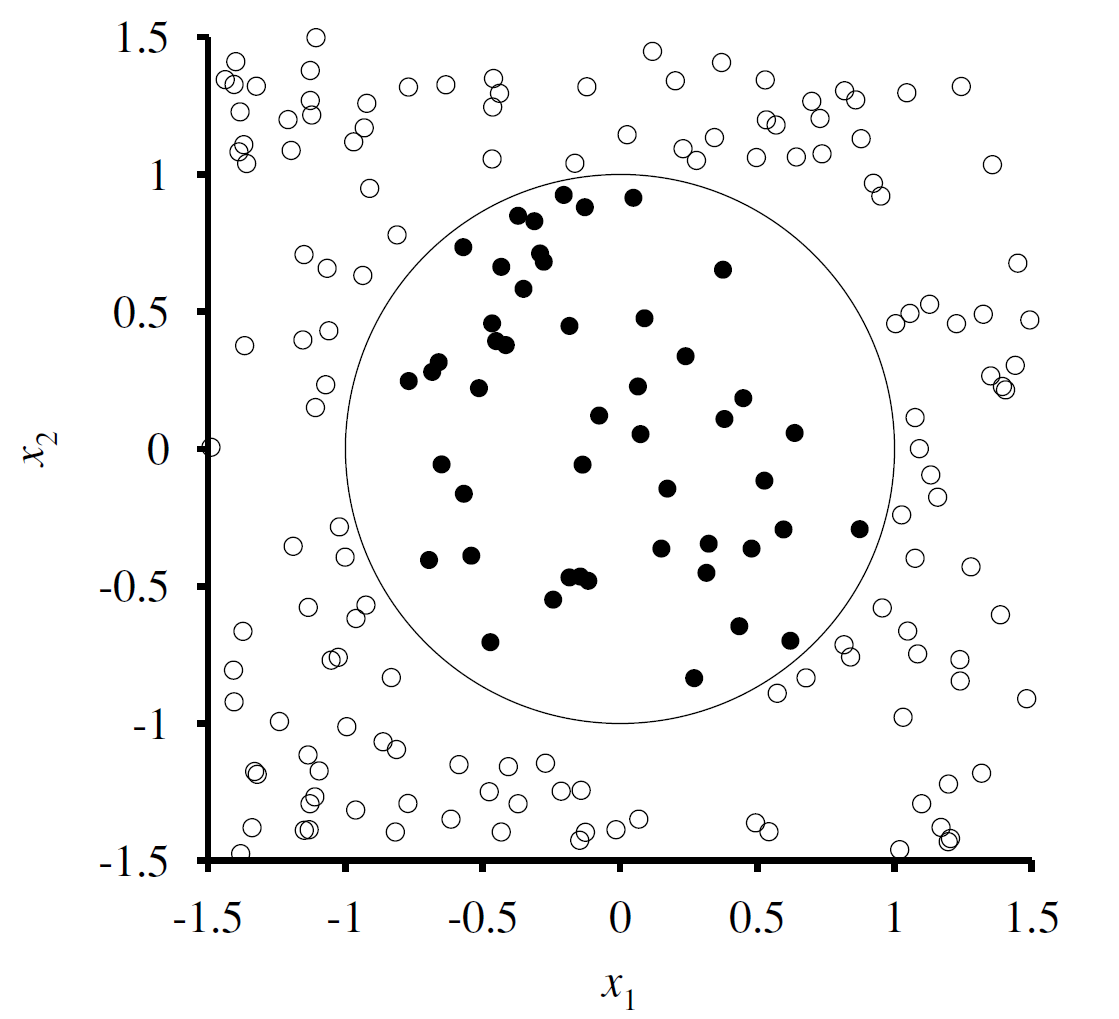
\includegraphics[width=\textwidth]{figures/svm_circular_decision_1.png}
    %     \caption{Datapoints with a circular decision boundary, resulting from the kernel trick.}
    %     \label{figure:kernel_decision_boundary}
    % \end{subfigure}
    % \begin{subfigure}{0.5\textwidth}
    %     \centering
    %     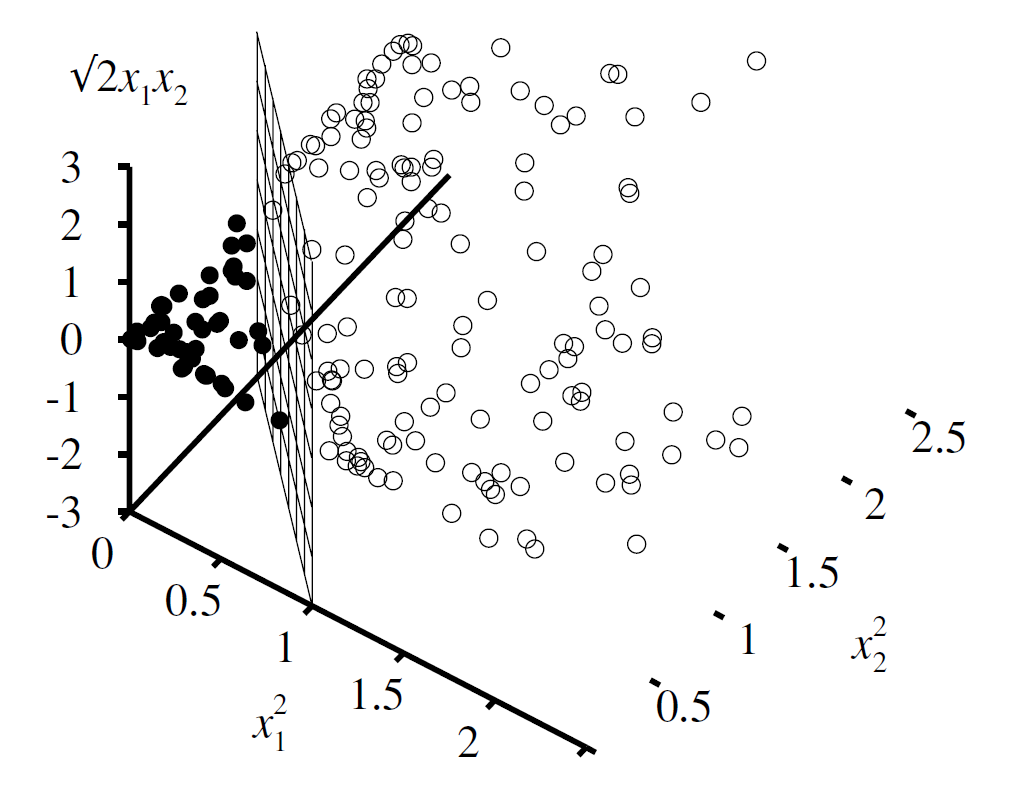
\includegraphics[width=\textwidth]{figures/svm_circular_decision_2.png}
    %     \caption{When mapped to a higher dimensional space, the datapoints become linearly seperable.}
    %     \label{figure:kernel_3d}
    % \end{subfigure}
    \caption{The kernel trick as visualised in \cite[p. 747]{Russel2016}}
    \label{figure:svm_kernel_trick}
\end{figure}

\subsection{Artificial Neural Networks}
Artificial neural networks imitate the structure of a brain, where each neuron receives input from other neurons, processes this information and passes it on to other neurons \cite[p. 727]{Russel2016}.
In artificial neural networks these neurons are represented as \textit{units}, which perform a mathematical operation on their input data.
This consists of first computing a weighted sum of its inputs and then applying a activation function $g$ on that sum, which determines whether the unit "fires" \cite[pp. 727-728]{Russel2016}:
\begin{equation}
    a_j=g\left(\sum_{i=0}^{n}w_{i,j}a_{i}\right)
    \label{equation:nn_unit_operation}
\end{equation}
Where $w_{i,j}$ is the weight, assigned to the input $a_i$.
A typical activation function is the sigmoid function defined by $\sigma(x)=\frac{1}{1+e^{-x}}$.
\begin{figure}[h]
    \centering
    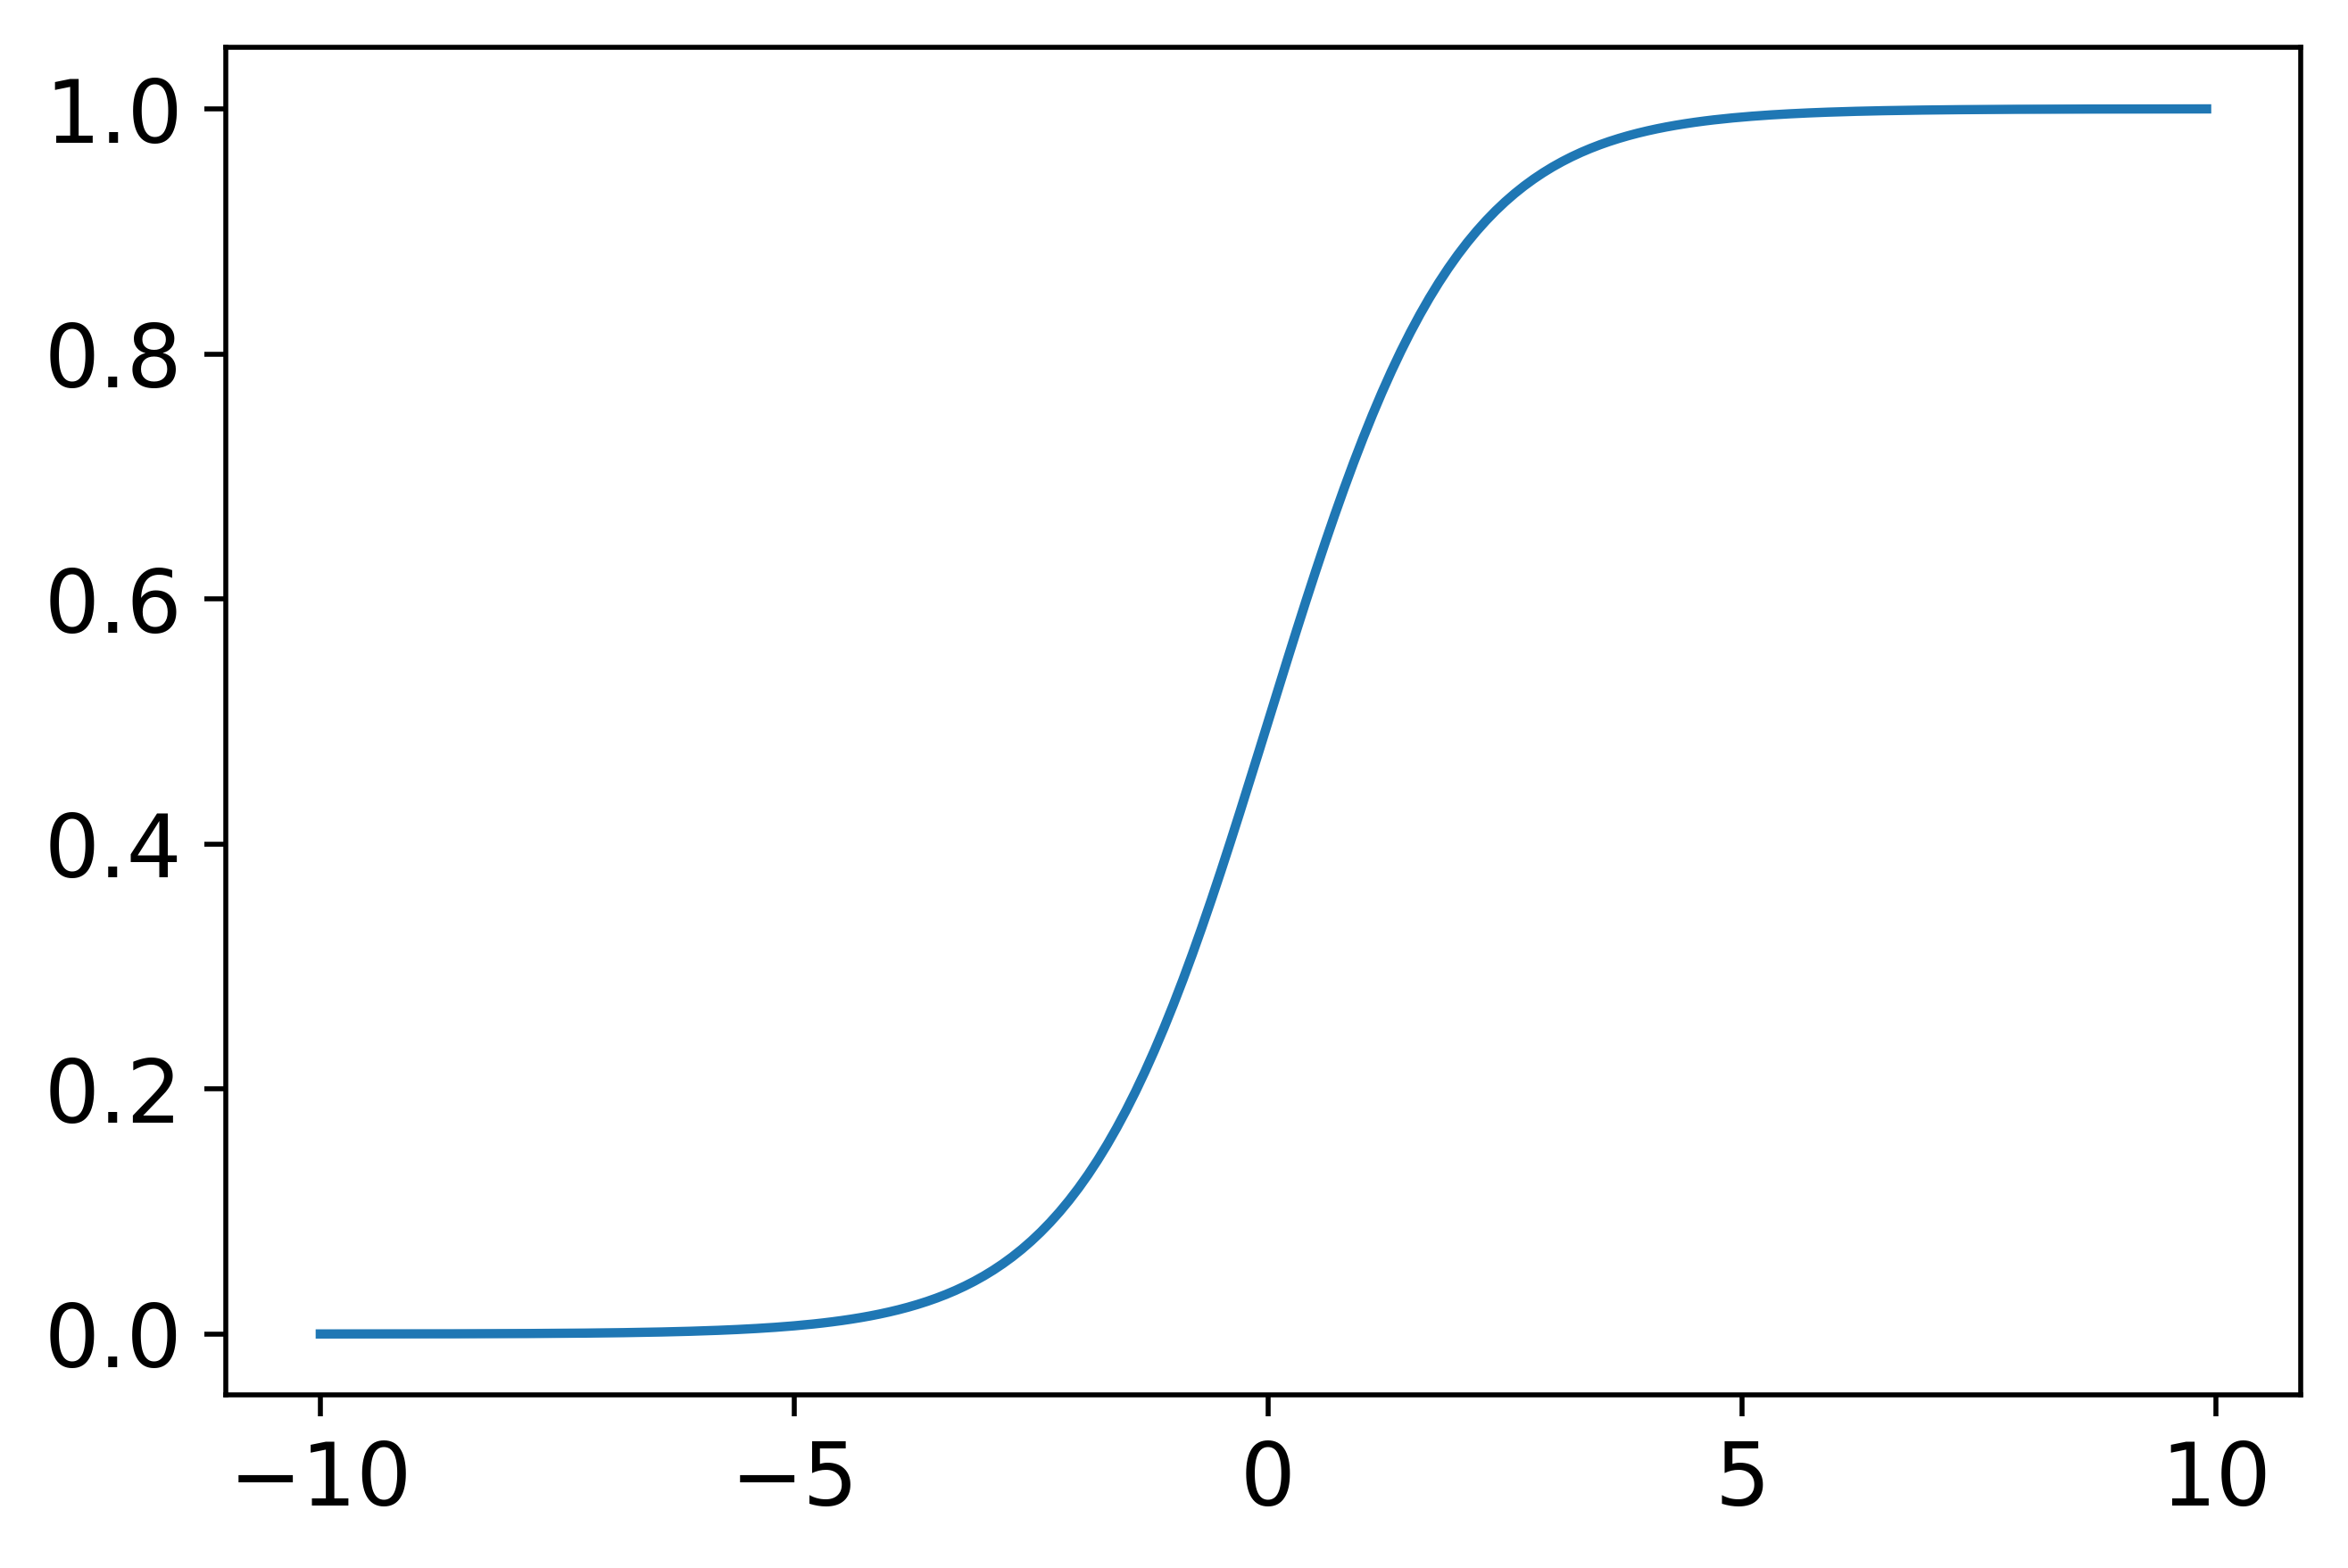
\includegraphics[width=0.5\textwidth]{figures/sigmoid.png}
    \caption{The sigmoid function.}
    \label{figure:sigmoid}
\end{figure}
As it can be seen in figure \ref{figure:sigmoid}, the sigmoid function results in values in the range from 0 to 1, which can be interpreted as the probability that the input belongs to one class.
The units are then structured into layers, with the simplest possible network having only two layers, one input and one output layer.
These simple networks are limited in their learning capabilities, that is why usually several hidden layers are added \cite[pp. 730-731]{Russel2016}.
% The input $a_j$ to a unit in such a hidden layer is itself the result of the computation with the function \ref{equation:nn_unit_operation}, therefore the whole network can mathematically be seen as a function applied to the input vector.
The network network predicts values by computing the output of each unit with function \ref{equation:nn_unit_operation} starting from the input layer.
The nodes in the subsequent layers use the same function to compute their outputs, however the input $a_i$ is the result of the computations on the previous layer.
The results of this computation on the output layer is the prediction of the network.
At training time, the units of the output layer then compute an error between the prediction it made and the actual value it should have predicted.
A common error metric is the squared-error loss $Loss_k$ on an output node $k$, which is defined in equation \ref{equation:squared_error_loss} \cite[p. 735]{Russel2016}.
\begin{equation}
    Loss_k=(y_k - a_k)
    \label{equation:squared_error_loss}
\end{equation}
With $a_k$ being the predicted value on output $k$ and $y_k$ being the actual value that should be predicted.
The aim is to minimize this loss with respect to all weights $w_{i,j}$ in the network $\frac{\partial Loss_k}{\partial w_{i,j}}$, which gives the gradient for the output node $k$.
The gradient can be computed with the \textit{back-propagation} algorithm.
The last layer computes an error term, based on the derivative of the loss function.
This error term is back-propagated to the previous layer, where each node again computes its own error, by summing the weighted errors of the subsequent nodes.
This is again repeated until the input layer is reached, then the weights between all nodes are updated based on the determined error terms \cite[p. 734]{Russel2016}.
% Auf nichtlinearität eingehen

A special class of neural networks are the \acp{RNN}, which have the ability to gather information from the order of the input items.
Therefore each input example consists of several \textit{timesteps}.
In case of report classification, like it is done in this thesis, the timesteps are the sentences of the report, which have a clear order to each other.
To process this sequential data the units in a \acs{RNN} (figure \ref{figure:rnn_unfolded}) are different to the units of a traditional feed-forward neural network.
\begin{figure}[h]
    \centering
    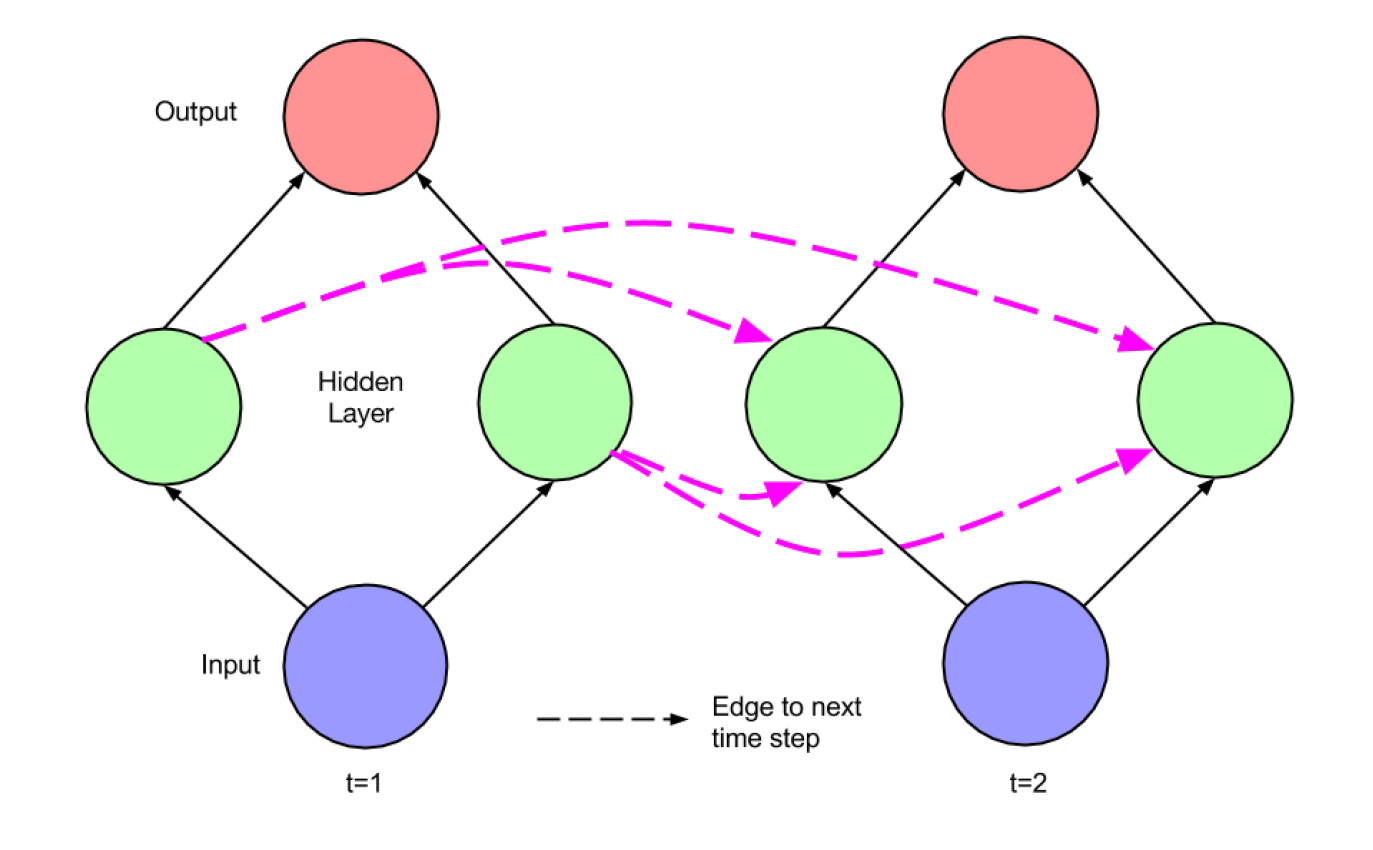
\includegraphics[width=0.5\textwidth]{figures/rnn_unfolded.png}
    \caption{The flow of the activations between two timesteps in an RNN as depicted in \cite[p. 12]{Lipton2015}.}
    \label{figure:rnn_unfolded}
\end{figure}
They have one input from the previous layer and a second one from the previous timestep.
On the output side they have an output for the next timestep and optionally also an output to the next layer \cite[p. 373]{Goodfellow2016}.
The training is done by computing the loss in the last timestep and propagating the loss back to the previous timestep.
A problem that occurs in standard \acp{RNN} is that the gradient decayes or increases exponentially while propagated back in time \cite[p. 13]{Lipton2015}.
A concept to avoid this problem is the \acs{LSTM}, which was proposed by \cite{Hochreiter1997}.
Figure \ref{figure:lstm_cell} shows the structure of a LSTM cell.
\begin{figure}[h]
    \centering
    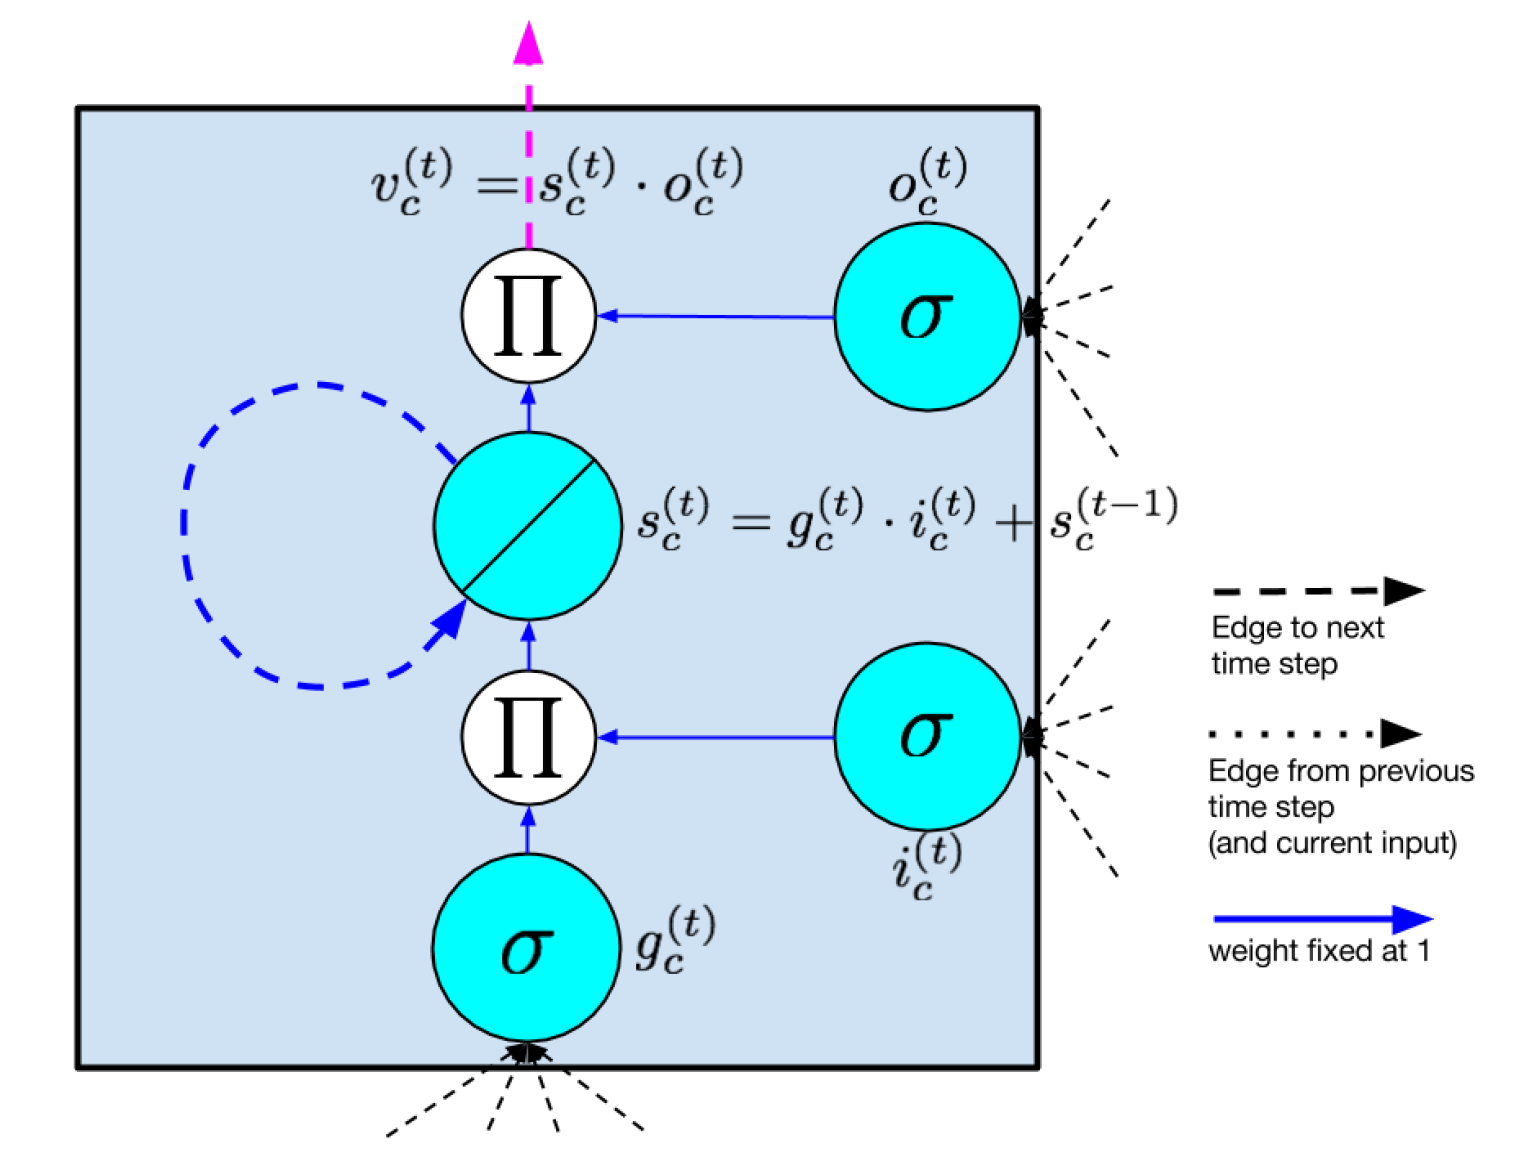
\includegraphics[width=0.5\textwidth]{figures/lstm_cell.png}
    \caption{A LSTM cell as depicted in \cite[p. 17]{Lipton2015}.}
    \label{figure:lstm_cell}
\end{figure}
Each of these units has an input gate which protects the unit against irrelevant input ($i_c$ in figure \ref{figure:lstm_cell}) and an output gate ($o_c$) which protects other units from possibly irrelevant content in the respective unit \cite[p. 6]{Hochreiter1997}.
Both, the \ac{RNN} as well as the \ac{LSTM}, have forms that also process the input sequence in the reverse order, the \ac{LSTM} is then called \ac{BLSTM}.

In this research the \ac{LSTM} implementation from Keras was used.
Although different network architectures were used, the general implementation with all used layer types is shown in listing \ref{py:lstm_implementation}.
\lstinputlisting[language=Python,caption={Implementation of a \acs{LSTM} in Keras.},label={py:lstm_implementation}]{listings/lstm.py}
The \texttt{LSTM} layers in listing \ref{py:lstm_implementation} consist of the just introduced \ac{LSTM} cells.
With the \texttt{return\_sequences} parameter the hidden states of all \ac{LSTM} cells on the respective layer can be used and the \texttt{go\_backwards} parameter reverses the order in which the sequential data is processed\footnote{\url{https://www.tensorflow.org/versions/r1.15/api_docs/python/tf/keras/layers/LSTM}}.
\texttt{Bidirectional} is a wrapper for a forward processing \ac{LSTM} layer and a backward processing \ac{LSTM} layer to create a \ac{BLSTM}\footnote{\url{https://www.tensorflow.org/versions/r1.15/api_docs/python/tf/keras/layers/Bidirectional}}.
With the \texttt{GlobalAveragePooling1D} layer the hidden states from the previous \ac{BLSTM} layer are averaged across the timesteps\footnote{\url{https://www.tensorflow.org/versions/r1.15/api_docs/python/tf/keras/layers/GlobalAveragePooling1D}}.
The \texttt{Dense} layer then is a layer with the regular feed forward units described at the beginning of this section \footnote{\url{https://www.tensorflow.org/versions/r1.15/api_docs/python/tf/keras/layers/Dense}}.

A key aspect is the usage of \texttt{None} in the first dimension of the \texttt{input\_shape} on line 11 in listing \ref{py:lstm_implementation}.
This dimension defines the number of time steps each input sample has.
Since each report has a different length, this value was set to \texttt{None}.
Even though the \ac{LSTM} can handle input with different time steps, on batch level it still requires to have input with a fixed number of time steps.
Therefore the reports need to be grouped by their lengths, which was accomplished with the \texttt{ReportSequence} class (Listing \ref{py:lstm_report_sequence}).
\lstinputlisting[language=Python,caption={The \texttt{ReportSequence} class creates batches with reports of same length.},label={py:lstm_report_sequence}]{listings/report_sequence.py}
This grouping is then used by calling the \texttt{fit\_generator} method on the model with an instance of the \texttt{ReportSequence} class in listing \ref{py:lstm_implementation} on line 26.
Similar to the previously described classifiers, a 5 fold cross-validation was used to select the best model architecture.

Now that the classification algorithms are introduced, one problem still remains:
The classifiers require the input to be a numerical vector.
Therefore the reports have to be converted to feature vectors.
This embedding step is described in the next section.


\section{Creating document embeddings}
\label{sec:creating_document_embeddings}
\subsection{Methods to create a document representation}
\label{subsec:methods_for_document_representation}
The task of the embedding step is to map a text of variable length to a vector of fixed length, which is necessary to train a classification algorithm.
The most basic approach for creating a text representation is the bag-of-words model.
For that a vocabulary is created which contains each word of a text corpus.
Each word in this vocabulary is represented by a vector with the dimensionality of the vocabulary size, having a $1$ on the entry at which the word is stored in the vocabulary and zeros on all other positions.
To create the representation of a document, the vectors of the words in the document are summed \cite[p. 13]{Grzegorczyk2018}.
Since a single document typically does not contain all words of the vocabulary this vector is sparse and an inefficient representation of the text.
This method also does not take into account that some words occur more frequently than others, which can be solved by mutiplying the term frequency with the inverse document frequency.
The resulting metric is called \textit{TF-IDF}:
\begin{equation}
    TF-IDF(t,d) = f_{t,d} \cdot log \frac{N}{n(t)}
    \label{equation:tf_idf}
\end{equation}
Where $f_{t,d}$ is the number of occurences of a term $t$ in a document $d$, $N$ the total number of documents and $n(t)$ the number of documents that contain the term $t$ \cite[p. 13]{Grzegorczyk2018}.

Another drawback of the word vectors in the bag-of-words model is, that it is not possible to determine similarity between different words.
Since they are all orthogonal to each other, "powerful", "strong" and "Paris" share the same similarity with each other \cite[p. 1]{Mikolov2014}.
This problem can be solved by using distributed vector representations, which can be created with the popular \textit{Word2Vec} implementation.
Word2Vec is a simple neural network with one hidden layer \cite[p. 22]{Grzegorczyk2018}.
It offers two algorithms to learn the word representations.
With the \ac{CBOW} algorithm the network predicts a word based on its surrounding words and with the \textit{skip-gram} algorithm the network tries to predict context words based on a center word \cite[pp. 4-5]{Mikolov2013}.
The word embeddings are then a result of maximizing the probabilities of these predictions \cite[p. 23]{Grzegorczyk2018}.
A simple approach for creating a document representation of these word embeddings would be to average all word vectors of the document.
Similar to the bag-of-words model with the term frequencies, this approach also does not respect the order of the words.
An extension to Word2Vec that creates a document representation is the \textit{Paragraph Vector} model \cite[p. 1]{Mikolov2014}, which is better known as the implementation \textit{Doc2Vec}.
For this model an additional paragraph representation is trained in parallel to the word representations \cite[p. 3]{Mikolov2014}.
The paragraph vector is incorporated in all word prediction contexts, therefore it captures the meaning of the whole document \cite[p. 3]{Mikolov2014}.

At the time of publication, \textit{Paragraph Vector} created state-of-the-art results in different sentiment tasks \cite[pp. 4-7]{Mikolov2014}, this thesis however, will use the modern language representation model \ac{BERT} to create the document embeddings.
In comparison to \textit{Paragraph Vector}, \ac{BERT} can use distant context words to the same extend as close words to create an embedding, whereas for the \textit{Paragraph Vector} model distant words contribute less to the embedding of a center word \cite[p. 4]{Mikolov2013}.
The ability to incorporate these long range relations is a result of the Transformer architecture which was proposed in \cite{Vaswani2017} and is the basis of \ac{BERT}.
\begin{figure}[h]
    \centering
    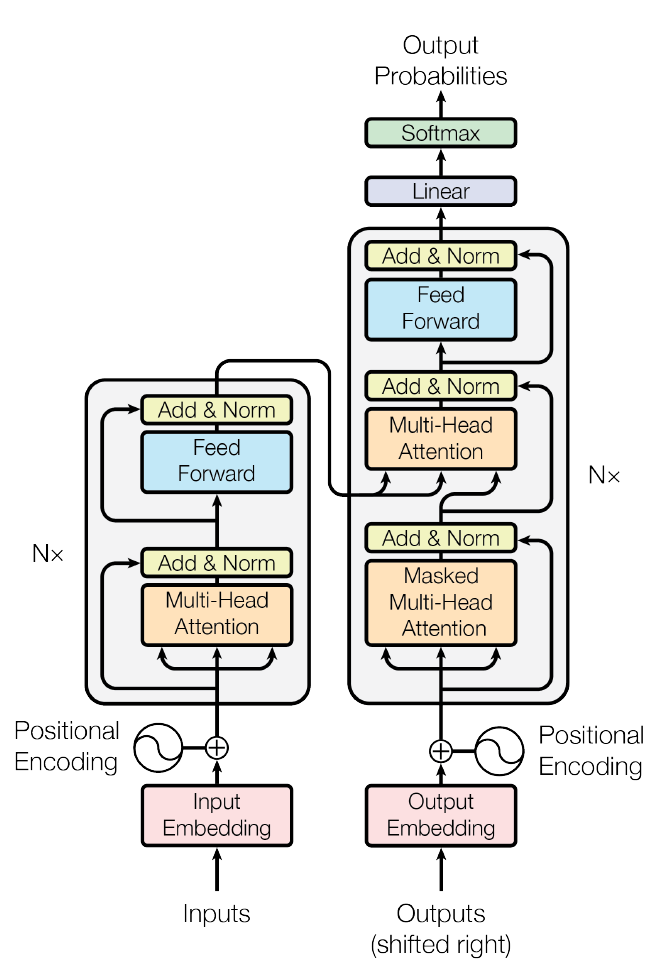
\includegraphics[width=0.5\textwidth]{figures/transformer_architecture.png}
    \caption{The Transformer architecture as proposed in \cite[p. 3]{Vaswani2017}.}
    \label{figure:transformer_architecture}
\end{figure}
From the pure application area, Transformer is really similar to \acp{RNN} or \acp{LSTM}, as it is also optimized for handling sequential data.
It uses an encoder-decoder structure with a self-attention mechanism.
The encoder maps an input sequence to a vector representation, which the decoder uses to create an output sequence.
This can be used for example for translation tasks, where a sentence from the original language is passed to the encoder and the decoder returns the translated sentence \cite[p. 392]{Goodfellow2016}.
Traditional encoder-decoder models use \acp{RNN} or \acp{LSTM} for the encoder and decoder with the vector representation being the final hidden state of the encoder \cite[p. 392]{Goodfellow2016}.
Enhancing these models with Attention, the hidden states of all encoder units can be used, with the focus on the most relevant states.
The Transformer architecture now relies purely on Attention and the sequential information is manually encoded in the data, which is labeled as \textit{Positional Encoding} in figure \ref{figure:transformer_architecture}.
Attention is accomplished by computing a weighted sum of the hidden states.
The weights are given by the similarity between the hidden states of the encoder, which are called the \textit{keys} and the most recent hidden state of the decoder, called the \textit{queries}.
This similarity between the queries and the keys is calculated as a dot-product, on which a softmax function is applied afterwards \cite[p. 4]{Vaswani2017}.
Between these weights and the \textit{values}, which are the hidden states of the encoder as well, another dot-product is calculated, giving the weighted sum.
In the Transformer model, this Attention mechanism is combined to a \textit{multi-head attention}.
The multi-head attention consists of multiple attention layers, each performing the attention on different linear projections of the query, key and value inputs and concatenating the results in the end \cite[pp. 4-5]{Vaswani2017}.
The advantage of the Transformer model is a high parallelization of the computation and the already mentioned capability to capture long range relations \cite[p. 2]{Vaswani2017}.
For \ac{BERT} the Transformer blocks depicted in figure \ref{figure:transformer_architecture} are stacked in multiple layers, with 12 layers in case of BERT\textsubscript{BASE} and 24 layers in case of BERT\textsubscript{LARGE} \cite[p. 3]{Devlin2018}.
Because of resource limitations, the BERT\textsubscript{BASE} model is used in this research.

Another important property of \ac{BERT} that can't be ignored, is that it can only process input text with a maximum sequence length of 512 tokens.
\textit{Tokens} are the entries in the vocabulary of \ac{BERT}.
Before \ac{BERT} can process the input text, it has to be tokenized.
In this tokenization step, each word from the input sequence is replaced with the longest token it can find in the \ac{BERT} vocabulary, that matches the word.
If no token matches the word exactly, the word is split in multiple tokens.
For example, the word \textit{discounted} is not in the vocab and the tokenizer therefore splits the word into the sub tokens \textit{discount} and \textit{\#\#ed}.
The restriction to a maximum sequence length of 512 tokens implies, that it is not possible to pass a whole business report to \ac{BERT}.
The segmentation into sentences with spaCy, that was described in section \ref{sec:data_preprocessing}, is part of solving this problem, however in some cases the resulting sentences are way shorter than the sequence length of 512 tokens.
Therefore the sentences are again concatenated until the maximum sequence length is reached.
For most applications working with \ac{BERT} involves two steps, a pre-training and a fine-tuning step.
In this research an additional feature extracting step was added which is described in section \ref{subsec:extracting_feature_vectors}.

\subsection{Pre-training}
In the \textit{pre-training} step, \ac{BERT} learns the general language structure which includes the positions of different words within a sentence and the relationship between successive sentences.
Since BERT is a language model with a deep architecture, bidirectional training of the word positions is not possible, because the network can trivially predict the target word. \cite[p. 4]{Devlin2018} %(<- Elaborate on here)
Therefore \cite{Devlin2018} decided to randomly mask out a number of words in the sentence and then predict the masked words.
\begin{figure}[h]
    \centering
    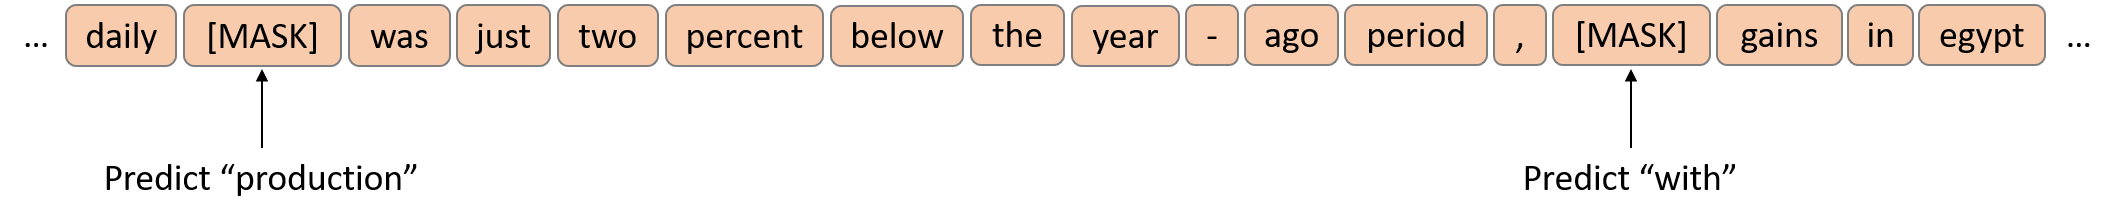
\includegraphics[width=1.0\textwidth]{figures/illustration_masked_lm.png}
    \caption{Illustration of the \textit{masked language model} pre-training task.}
    \label{figure:masked_lm}
\end{figure}
The masking of the words is done by a tokenizer, which was also released with \ac{BERT}.
For representing the masked words, the special token \texttt{[MASK]} is used.
Another special token is the \texttt{[CLS]} token, which is prepended to each input sequence and holds the meaning of this sequence after the \textit{fine-tuning} procedure \cite[p. 4]{Devlin2018}.
The whole task of predicting masked words based on their contexts is called \textit{masked language model} \cite[p. 4]{Devlin2018}.
The second task during pre-training is the binary \textit{next sentence prediction}.
For that, given a sentence \textit{A}, the sentence \textit{B} is either the actual successive sentence or a randomly chosen sentence from the training corpus.
\ac{BERT} has to predict then, whether the sentence is the successive sentence or not.

Because \ac{BERT} is using Tensorflow as a backend, it expects the input data to be in the TFRecord file format.
TFRecord is a binary file format, which contains the tokenized text and the tokens that are masked.
Because the creation of each TFRecord file takes a few seconds, the dataset is again split to optimize the processing with multiple cores, as it can be seen in Listing \ref{py:split_data_and_spawn_processes}.
\lstinputlisting[language=Python,caption={The dataset is split to optimize the TFRecord creation on multicore systems.},label={py:split_data_and_spawn_processes}]{listings/split_data_and_spawn_processes.py}
The \texttt{\_handlePretrainingDataCreation()} function, which is provided as as a callback to the \texttt{Process}, is mostly similar to the \texttt{main()} function of \texttt{create\_pretraining\_data.py} from the official \ac{BERT} repository\footnote{The official \ac{BERT} repository on GitHub: \url{https://github.com/google-research/bert}}.
It was modified, so it creates the TFRecord files for multiple input files at once.

The actual training of \ac{BERT} was done with the script in listing \ref{py:run_pretraining}.
\lstinputlisting[language=Python,caption={\ac{BERT} pre-training.},label={py:run_pretraining}]{listings/run_pretraining.py}
Again most of the source code is similar to the \texttt{main()} function of \texttt{run\_pretraining.py} from the official \ac{BERT} repository.
One change that was made, was to set the number of checkpoints, that are created during training, to 30 as opposed to 5 as default.
These checkpoints were later used to validate the model.
The validation step was also moved to a seperate script to evaluate the model for every training checkpoint.
This is accomplished by iterating over the created checkpoints and calling the evaluation code from \ac{BERT} for each of them.
In the original source code only the final model was evaluated.
The results are appended to a Pandas DataFrame, which is saved as a \ac{CSV} file in the end.

\subsection{Fine-Tuning}
\label{subsec:fine_tuning}
The \textit{fine-tuning} step is used to optimize \ac{BERT} for a specific task.
This can be a task like question answering or sentence classification \cite[pp. 5-7]{Devlin2018}.
Even though the final goal is to classify the business reports and not every sentence on its own, the fine-tuning is essential so that the \texttt{[CLS]} token holds a good representation of the sentence\footnote{This hint was mentioned in \texttt{extract\_features.py} on lines 237-239 \url{https://github.com/google-research/bert/blob/fe354751d7de010f60d362ae8d9343849ec39456/extract_features.py}}.
Since the final aim is to classify each business report, the most similar task was selected for fine-tuning, which is the sentence classification.
In difference to the pre-training, the sequences for fine-tuning need a label.
Since each input sequence to \ac{BERT} is a part of a larger report, the sequences "inherit" their label from this report.
Therefore a sentence of a \textit{positive} report is also labeled \textit{positive} and a sentence of a \textit{negative} report is also labeled as \textit{negative}.
Of course this approach seems wrong on the first glance, since a positive report can also contain negative sentences and vice versa.
However one could also re-interpret the classification task as follows:
Instead of saying that the label indicates whether a sentence is a \textit{positive} or \textit{negative} sentence, it can also be interpreted as indicating whether the sentence belongs to a \textit{positive} or \textit{negative} report.
Section \ref{sec:fine_tuning_results} shows how this approach affects fine-tuning.

As opposed to the pre-training, the creation of the TFRecord files was part of the training script for fine-tuning.
Therefore every training run was delayed, because the TFRecord files were generated first.
The call to the \texttt{file\_based\_convert\_examples\_to\_features} function, which creates the TFRecord files was therefore moved to another script (Listing \ref{py:convert_to_tfrecord}).
\lstinputlisting[language=Python,caption={Creates the TFRecord files for fine-tuning.},label={py:convert_to_tfrecord}]{listings/convert_to_tfrecord.py}
This allows to train the model without waiting for the creation of the TFRecord files.
Similar to the changes made for pre-training, the number of checkpoints to save was also increased and the validation of the model was moved to a second script.

\subsection{Extracting feature vectors}
\label{subsec:extracting_feature_vectors}
After the fine-tuning is accomplished, the \texttt{[CLS]} token at the start of each sequence holds information about the class of the sequence.
This information can be retrieved by accessing the hidden states of the Transformer blocks in the last layer of the model.
Listing \ref{py:extract_features} shows a snippet of the \texttt{extract\_features.py} script.
\lstinputlisting[language=Python,caption={Accesses the hidden states from the transformer layers.},label={py:extract_features}]{listings/extract_features.py}
The official implementation allows to access the hidden states from all layers of the model, however for this thesis only the last layer is used.
For that the \texttt{layer\_indexes} variable which is passed to the \texttt{model\_fn\_builder} is set to -1.
Therefore the hidden states of this layer can be accessed by \texttt{result["layer\_output\_0"]} on line 21.
In theory the \texttt{result} dictionary also includes \texttt{layer\_output\_1, layer\_output\_2, ...}, but the \texttt{layer\_indexes} limits the results.
In the list comprehension on line 23 \texttt{layer\_output[0]} only the hidden states for the first token, the \texttt{[CLS]} token, is accessed.
The \texttt{for} loop is necessary because the \texttt{predict} method returns an iterator, where each element represents the hidden states for one line of the input file.
As a summary it can be said, that this implementation only takes the hidden states from the last layer for the first token, while the official implementation takes the hidden states for all tokens from possibly all layers.

Because of the limitation of \ac{BERT} that it can only process sequences with a maximum length of 512 tokens, many embedding vectors result for each report.
For the \ac{BLSTM} the single sequence embeddings give the timesteps for each sample.
The Naive Bayes, \ac{KNN} and \ac{SVM} however, need a single vector representation for each report, therefore the sequence embeddings are averaged per report.

\section{Other used techniques}
\subsection{Cross-Validation}
\label{subsec:cross_validation}
Cross-validation is a method to estimate the prediction accuracy of a model for a unknown dataset \cite[p. 241]{Hastie2009}.
For that a training dataset is split in $K$ equally sized parts.
$K-1$ of these parts are then used to train the model and the $k$th part is used to evaluate the model.
This is repeated for $k=1,2,...,K$ and the resulting accuracies are averaged \cite[p. 242]{Hastie2009}.
The averaged accuracy is used to optimize the model:
The hyperparameters of the model are changed so that the averaged accuracy is maximized \cite[p. 242]{Hastie2009}.
One drawback of the method is that it multiplies the time to train and evaluate the model approximately by the value of $K$ \cite[p. 242]{Hastie2009}.

For this research 5-fold cross-validation was used for the Naive Bayes, \ac{KNN}, \ac{SVM} and the \ac{BLSTM}.
The hyperparameters for the \ac{BERT} pre-training and fine-tuning were determined without cross-validation, because \ac{BERT} itself is quite computational expensive.

\subsection{Learning and validation curve}
This thesis uses learning curves to visualise the learning progress of the machine learning models.
A learning curve is a line chart that shows the accuracy of a machine learning model depending on a second variable, like the training dataset size or the number of epochs a neural network trained \cite[pp. 702-703]{Russel2016}.
It can give evidence about whether the model would improve its performance if more data was available or the number of epochs was increased.
In this thesis, the accuracies of the Naive Bayes, \ac{KNN} and \ac{SVM} are indicated depending on the size of the training dataset and for the \ac{BLSTM} the accuracies are indicated depending on the number of epochs.
For \ac{BERT} the horizontal axis shows the number of training steps, which is a comparable measurement with the number of epochs (Chapter \ref{ch:experiments}).

Validation curves are used to find the best hyperparameters of a model.
They show the accuracy of the model depending on different values of this hyperparameter, that can be for example the number of $K$ in the case of the \ac{KNN} or the value of $C$ for a linear \ac{SVM}.
The best value is then selected by choosing the model that reached the highest validation accuracy \cite[p. 711]{Russel2016}.

In this thesis both of the curves are created in combination with cross-validation.
\begin{figure}[h]
    \begin{subfigure}{0.5\textwidth}
        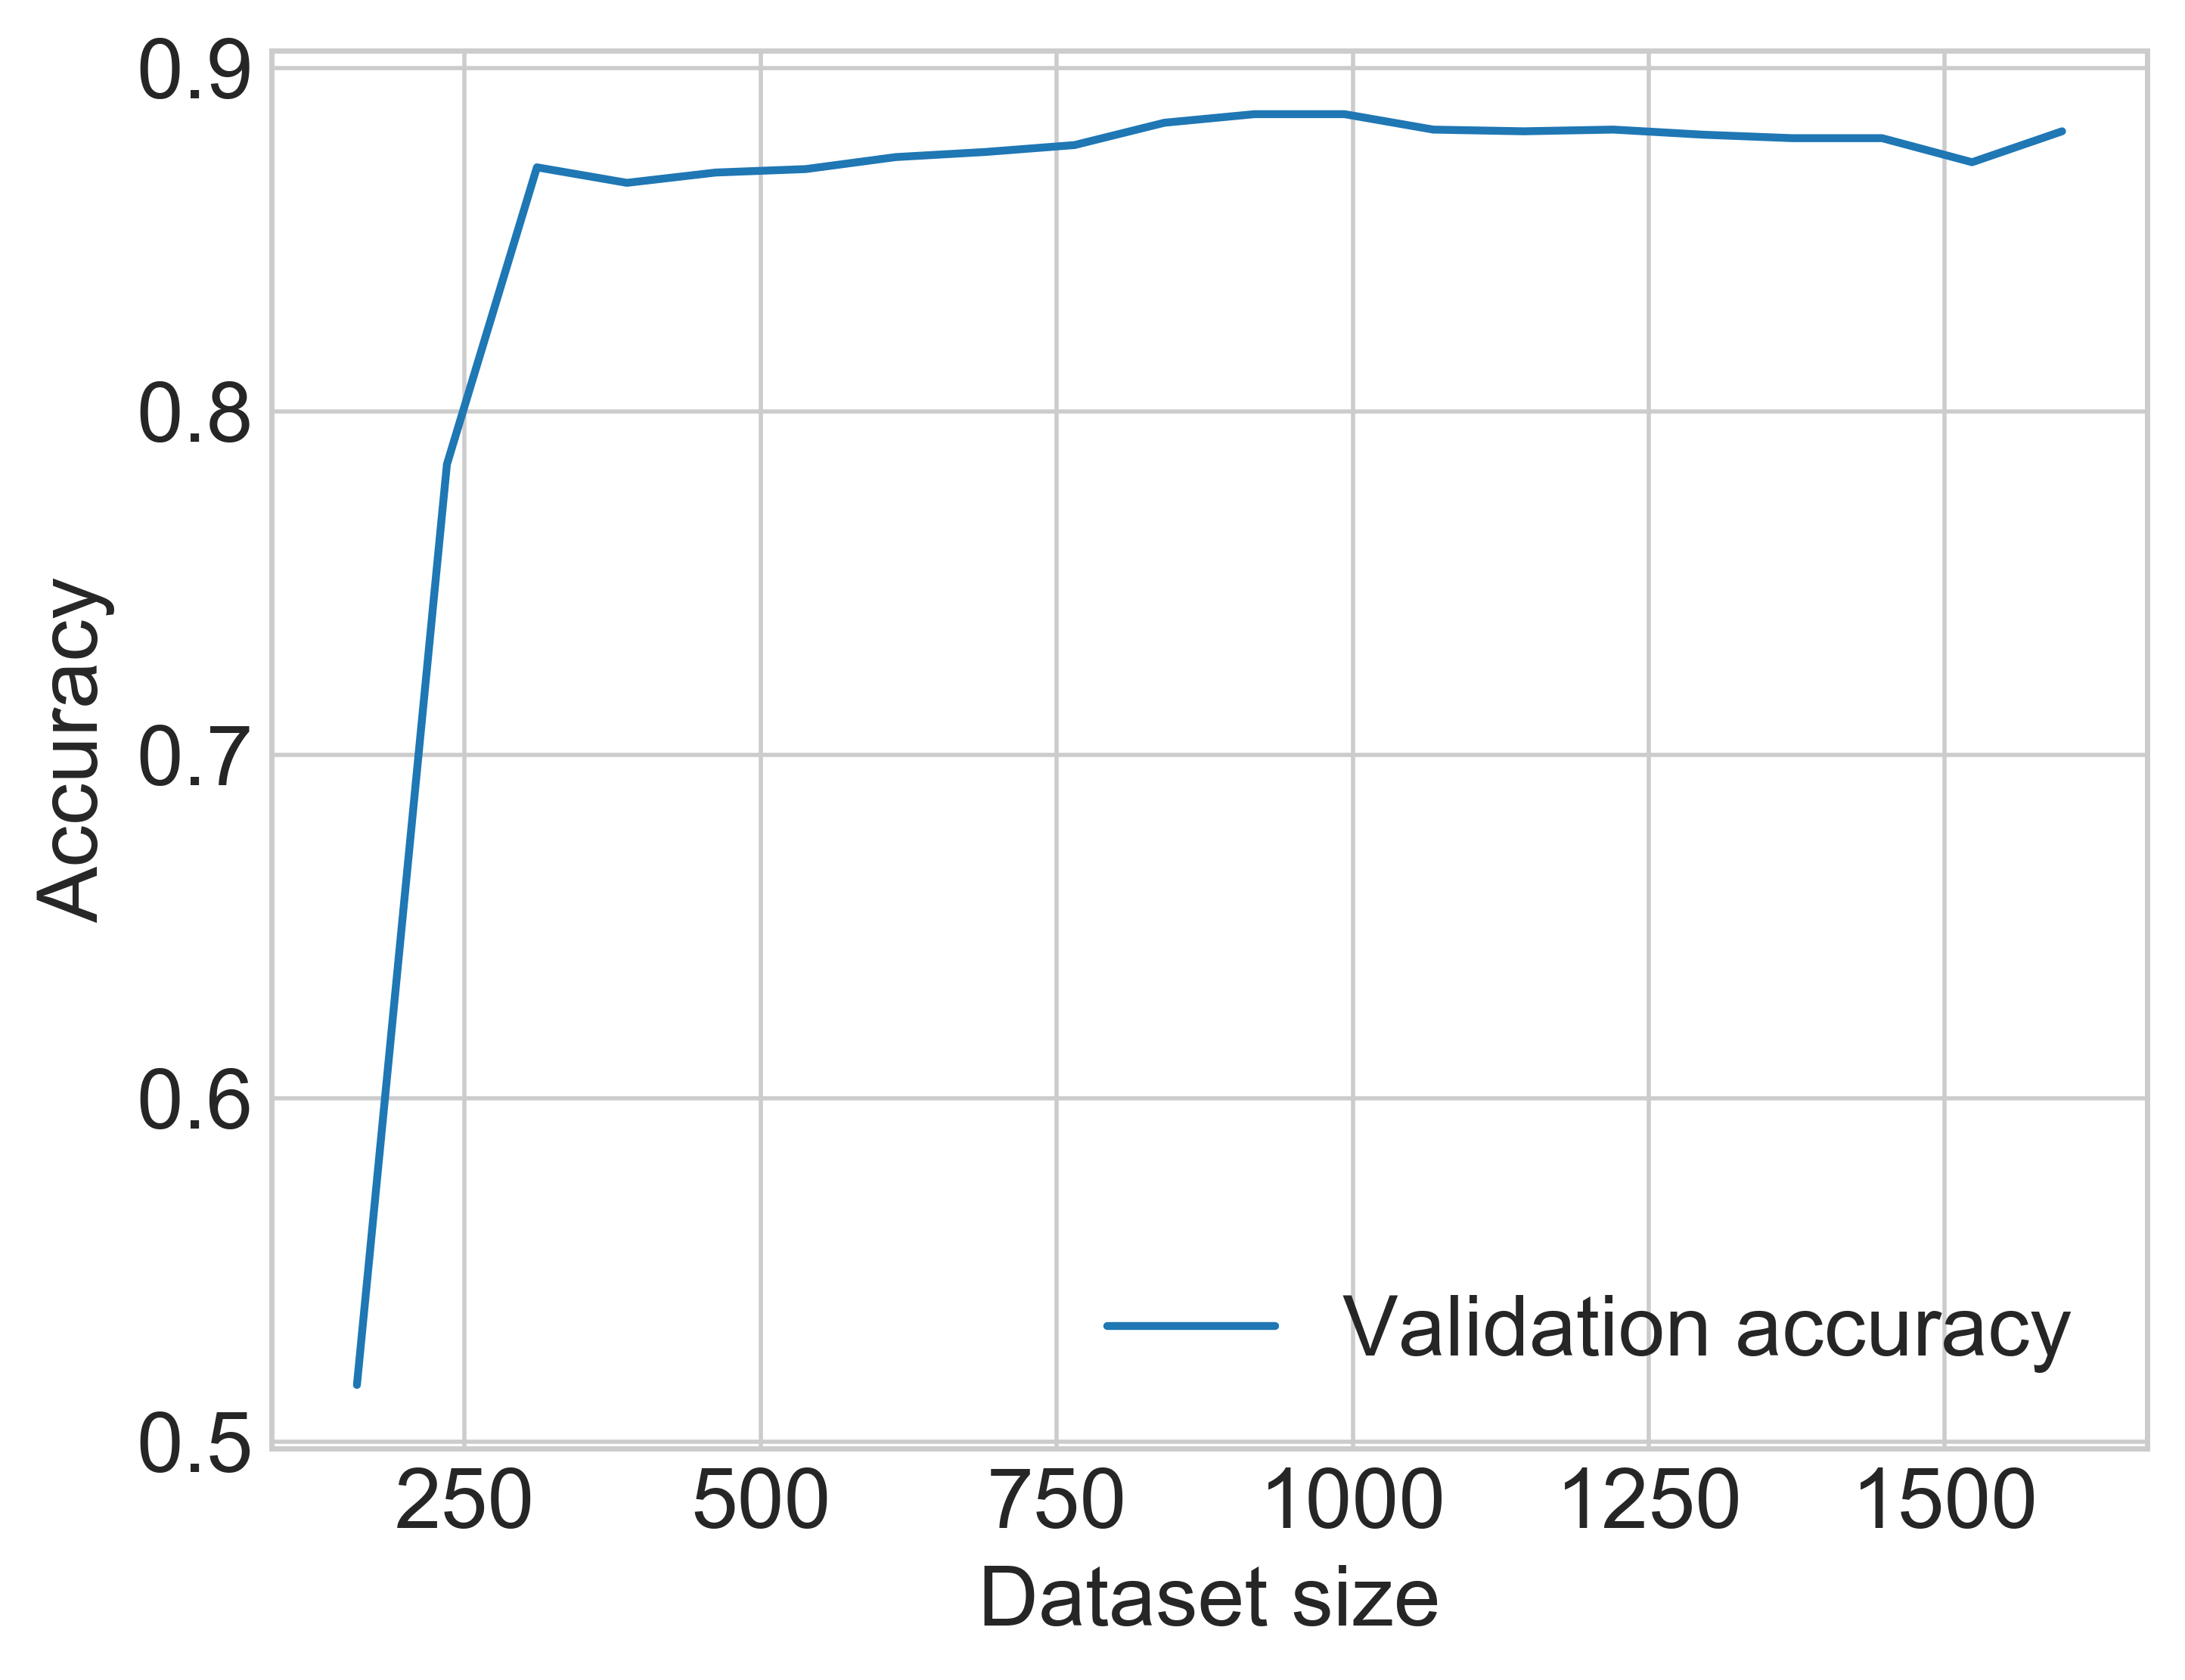
\includegraphics[width=\textwidth]{figures/knn_sample_learning_curve.png}
        \caption{The learning curve shows the accuracy depending on the training dataset size.}
        \label{figure:sample_learning_curve}
    \end{subfigure}
    \begin{subfigure}{0.5\textwidth}
        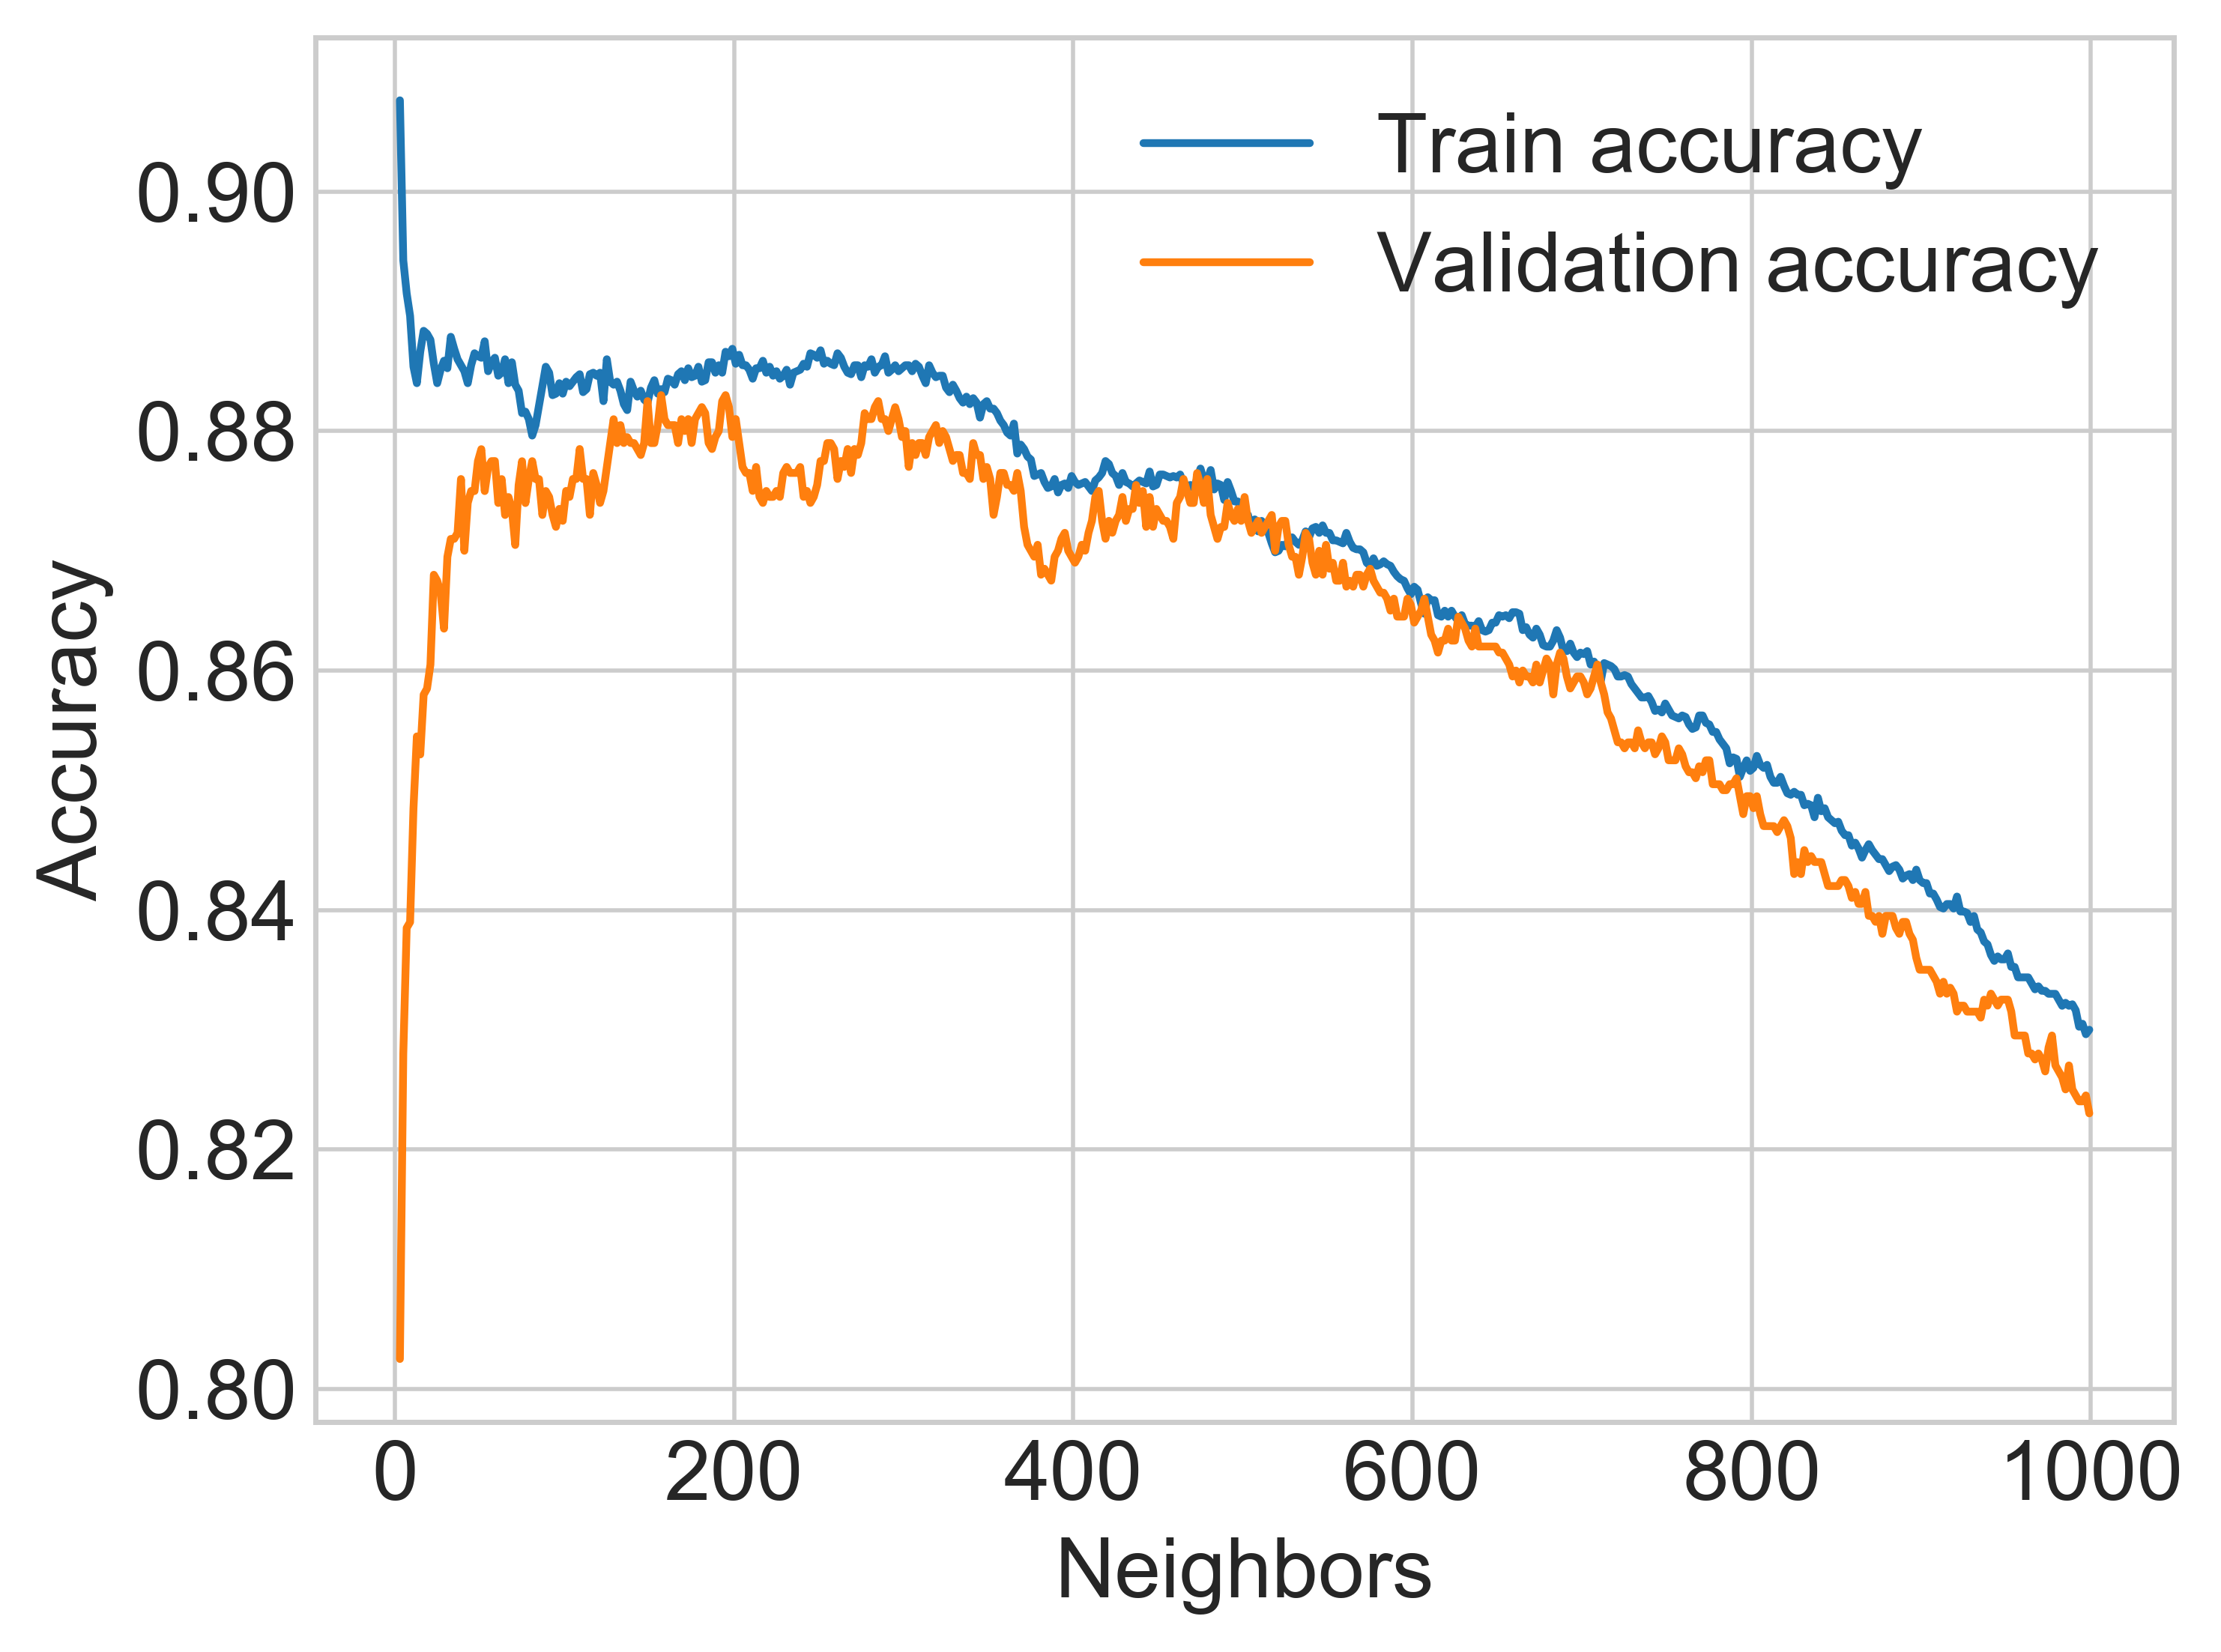
\includegraphics[width=\textwidth]{figures/knn_sample_validation_curve.png}
        \caption{The validation curve shows how a change in the value of a hyperparameter affects the accuracy of the model.}
        \label{figure:bert_pretraining_learning_512_nsp}
    \end{subfigure}
    \caption{Sample learning and validation curves of a \ac{KNN} classifier.}
    \label{figure:bert_pretraining_learning_512}
\end{figure}


\subsection{\acl{PCA}}
\acl{PCA} is a methode to reduce the dimensionality of a dataset with loosing as little information as possible.
In this thesis \ac{PCA} is used to obtain a two dimensional representation of the data, which can then be visualised.
Mathematically the \ac{PCA} can be seen as the projection of a data matrix $X$ to a target matrix $Y$ with other basis vectors (equation \ref{equation:pca_projection}) \cite[p. 3]{Shlens2014}.
\begin{equation}
    PX=Y
    \label{equation:pca_projection}
\end{equation}
For the application of this thesis $X$ is a $m\times n$ matrix where each column contains the hidden states for the business report.
$Y$ is a $m\times n$ matrix as well, with the special property, that the rows are sorted by their variances, with the highest variance in the first row \cite[p. 5]{Shlens2014}.
To accomplish this, the covariance matrix $C_X$ of $X$ is computed.
If the row entries of $X$ have a zero mean, the covariance matrix is given by $C_X=\frac{1}{n}XX^T$ \cite[p. 5]{Shlens2014}.
If the mean is not zero, each value has to be subtracted by the corresponding row mean first.
Then the eigenvectors of $C_X$ are computed, which form the rows of the projection matrix $P$ \cite[p. 6]{Shlens2014}.
Another way of solving the \ac{PCA} is to use singular value decomposition, this is described in detail in \cite[p. 7]{Shlens2014}.


% This is done by fitting a hyperplane with dimension $q \leq p$ into the featurespace with dimension $p$ that minimises the squared error to the data points.
% For practical usage the dimension $q$ of the hyperplane is typically 2 or 3.
% For $q=2$, the hyperplane is a twodimensional plane on which the values are projected and can then be visualised.